%%%%%%%%%%%%%%%%%%%%%%%%%%%%%%%%%%%% Slide %%%%%%%%%%%%%%%%%%%%%%%%%%%%
%%%%%%%%%%%%%%%%%%%%%%%%%%%%
\begin{frame}[fragile,t]{Spaces}
	\begin{itemize}
		\item If you want to add extra white space (or subtract some) you can use the \verb|\vspace{xyz}| and \verb|\hspace{xyx}| commands
		\begin{itemize}
			\item You can use units of ``pts'' (as in font size), ``in'' for inches, or ``cm'' for centimeters
			\item Example: \verb|\vspace{0.2in}| for $0.2$ inch or \verb|\vspace{12pt}| for 12 points
		\end{itemize}
\vspace{0.1in}
		\item \verb|\vspace{xyz}| controls the vertical spacing
		\begin{itemize}
\vspace{0.05in}
			\item Using positive values adds extra white space between lines
\vspace{-0.05in}
			\item Using negative values shrinks the white space between lines/objects
			\item You can also add ``\verb|\\|'' to the end of a line to force a new line
		\end{itemize}
\vspace{0.1in}
		\item \verb|\hspace{xyz}| controls the horizontal spacing
		\begin{itemize}
			\item \hspace{0.2in} Using positive values pushes text right
			\item \hspace{-0.25in} Using negative values pushes text left
			\item You can also add an extra spacebar using a backslash ``$\backslash$''
		\end{itemize}
	\end{itemize}
\end{frame}


%%%%%%%%%%%%%%%%%%%%%%%%%%%%%%%%%%%% Slide %%%%%%%%%%%%%%%%%%%%%%%%%%%%
%%%%%%%%%%%%%%%%%%%%%%%%%%%%
\begin{frame}[fragile,t]{Input Files}
	\begin{itemize}
		\item When dealing with large presentations, it can become difficult to use a single .tex file
		\begin{itemize}
			\item Instead use \verb|\input{filename}| to break up one file into several
		\end{itemize}
\vspace{0.1in}
		\item I use a single ``root'' file titled ``main.tex'' that calls several input files, labeled something like ``sec\_blahblahblah.tex''
		\item Nothing new is needed in the input file - no special ``begin{}'' etc - just start making frames as you would otherwise
		\item All you need is a command \verb|\input{sec_blahblahblah}| in the root folder - it will include all the frames in ``sec\_blahblahblah'' before the next set of slides
		{\tiny
		\begin{lstlisting}
\begin{frame}[t]{This is the 1st slide}
	Blah blah blah
\end{frame }
\input{sec_TenSlides} %insert the 10 slides specified by the file ``sec_TenSlides.tex''
\input{sec_FiveSlides} %insert the 5 slides specified by the file ``sec_FiveSlides.tex''
\begin{frame}[t]{This is the 17th slide}
	Blah blah blah
\end{frame }
		\end{lstlisting}
		}
	\end{itemize}
\end{frame}

%%%%%%%%%%%%%%%%%%%%%%%%%%%%
\addtocounter{framenumber}{-1}
\begin{frame}[t]{Input Files}
	\begin{center}
		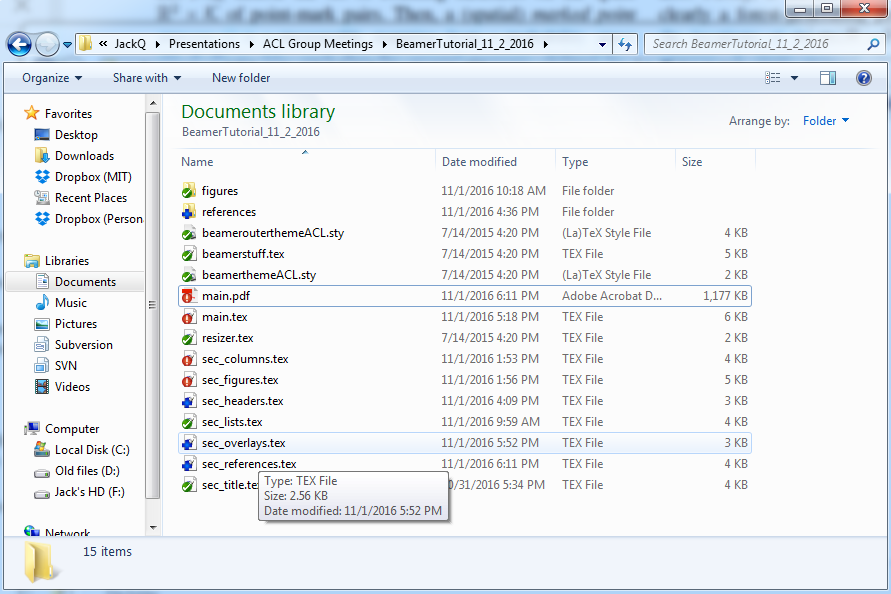
\includegraphics[width=0.95\columnwidth]{figures/folderView.png}
	\end{center}
\end{frame}


%%%%%%%%%%%%%%%%%%%%%%%%%%%%%%%%%%%% Slide %%%%%%%%%%%%%%%%%%%%%%%%%%%%
%%%%%%%%%%%%%%%%%%%%%%%%%%%%
\begin{frame}[fragile,t]{Math Equations/Symbols}
	\begin{itemize}
		\item No modifications have to be made to write mathematical equations or symbols while operating in beamer
		\begin{lstlisting}
\begin{frame}[t]{Math Equations}
	You can still add math symbols to sentences 
	by using dollar signs\\
	like this $1 + 1 = \alpha$ \\
\vspace{0.2in}
	And use equations in the same way like
	\begin{equation}
		1 + 1 = \alpha
	\end{equation}
\end{frame }
		\end{lstlisting}
		\item Check out \href{https://en.wikibooks.org/wiki/LaTeX/Mathematics}{HERE} and \href{http://www.colorado.edu/physics/phys4610/phys4610_sp15/PHYS4610_sp15/Home_files/LaTeXSymbols.pdf}{HERE} if you don't know LaTeX math
	\end{itemize}
\end{frame}


%%%%%%%%%%%%%%%%%%%%%%%%%%%%%%%%%%%% Slide %%%%%%%%%%%%%%%%%%%%%%%%%%%%
%%%%%%%%%%%%%%%%%%%%%%%%%%%%
\begin{frame}[fragile,t]{Pop-Up Text Blocks}
	\begin{itemize}
		\item You can hard code pop-up text blocks
		\begin{itemize}
			\item You'll have to include the following code immediately following the other packages at the beginning of the document		
			{\tiny
			\begin{lstlisting}
\usepackage[absolute,overlay]{textpos} 
\newenvironment{myfootnote}[3]{%
\begin{textblock*}{#3}(#1,#2) 
\tiny\begingroup\color{blue!50!black}}{\endgroup\end{textblock*}}
			\end{lstlisting}
			}
			\item Then you'll create a textbox using
			{\tiny
			\begin{lstlisting}
\only<2->{
\begin{textblock*}{0.99\textwidth}(0.05\textwidth,37ex) 
	\begin{block}{Textbox title}
		Whatever you say in the textbox
	\end{block}
\end{textblock*}
}
			\end{lstlisting}
			}
			\begin{itemize}
				\item The \verb|\only<2->| command makes the textbox only popup in the second frame
				\item The line \verb|\begin{textblock*}{0.99\textwidth}(0.05\textwidth,37ex)| sets \{width of textblock\}(distance from left of page, distance from top of page)
			\end{itemize}
		\end{itemize}
	\end{itemize}
	\only<2->{
	\begin{textblock*}{0.99\textwidth}(0.05\textwidth,10ex) 
		\begin{block}{Textbox title}
			\begin{itemize}
				\item It does something like this!
				\item Notice that I can do all the other commands (like bulleted lists) in here too!
			\end{itemize}
		\end{block}
	\end{textblock*}
	}
\end{frame}
	
%%%%%%%%%%%%%%%%%%%%%%%%%%%%%%%%%%%% Slide %%%%%%%%%%%%%%%%%%%%%%%%%%%%
\subsection{Adding Movies}
%%%%%%%%%%%%%%%%%%%%%%%%%%%%
\begin{frame}[t]{Adding Movies}
	\begin{itemize}
		\item You can also add movies to beamer presentations
		\begin{enumerate}
			\item Embed Youtube links
			\item Embed local videos stored on your hard drive
		\end{enumerate}
\vspace{0.2in}
		\item I took these slides from my earlier presentation
		\begin{itemize}
			\item I didn't include local videos
			\item You can find that complete presentation here \url{svn://acl.mit.edu/acl/ACL_Beamer_Template/movie_making.tex}
		\end{itemize}
	\end{itemize}
\end{frame}

%%%%%%%%%%%%%%%%%%%%%%%%%%%%%%%%%%%%% New slide
\begin{frame}[t]{Notes}
	\begin{itemize}
		\item \textbf{Intro}: you should use this as a template for embedding videos.  Copy and paste it into your code as necessary
\vspace{12pt}
		\item I've tested this on both Windows and Ubuntu
		\begin{itemize}
			\item Depending on your compiler, you might not be able to see the videos in your compiler's display, but you can view it when you open it in Adobe Reader/Acrobat
		\end{itemize}
\vspace{12pt}
		\item \textbf{However}, I have not been able to get the videos to display properly in Ubuntu
		\begin{itemize}
			\item It correctly compiles - the videos are embedded, but the presentation software can't display it
			\item I've tried Adobe Reader 9, Okular in Ubuntu but have not been able to get videos to display properly
			\item Feel free to edit this if you do get it to work!
		\end{itemize}
	\end{itemize}
\end{frame}

%%%%%%%%%%%%%%%%%%%%%%%%%%%%%%%%%%%%% New slide
\begin{frame}[t]{Notes}
	\begin{itemize}
		\item Two ways to embed videos in your presentation:
		\begin{enumerate}
			\item Youtube (or whatever else) links embedded in the player
			\item Local files on your hard drive
		\end{enumerate}
\vspace{12pt}
		\item This uses the media9 package.  You have to make sure it's added - see line 18 of the TeX code
\vspace{24pt}
		\item Start with Youtube videos
	\end{itemize}
\end{frame}


%%%%%%%%%%%%%%%%%%%%%%%%%%%%%%%%% New slide - THIS IS A YOUTUBE LINK EXAMPLE
\begin{frame}[t]{Youtube Video}
	\begin{itemize}
		\item This is the baseline example
	\end{itemize}
	\begin{figure}
	\centering
\includemedia[
	    width=0.9\paperwidth,height=0.5\linewidth,
	    activate=pageopen, %Load the video (but you'll have to click the button to start)
	    flashvars={autoPlay=true}
	        ]{}{https://www.youtube.com/v/opsmd5yuBF0} %URL of video
        \end{figure}
\end{frame}

%%%%%%%%%%%%%%%%%%%% New slide - THIS IS A YOUTUBE LINK EXAMPLE - BETTER BECAUSE IT REMOVES TITLEBAR AND WHATNOT
\begin{frame}[t]{Youtube Video}
	\begin{itemize}
		\item This removes the title bar from the top of the video
	\end{itemize}
	\begin{figure}
	\centering
\includemedia[
	    width=0.9\paperwidth,height=0.5\linewidth,
	    activate=pageopen, %Load the video (but you'll have to click the button to start)
	    flashvars={modestbranding=1 % no YT logo in control bar
        		&autohide=1 % controlbar autohide activated
        		&showinfo=0 % no title and other info before start
        		&rel=0 % no related videos after end}
        		}
	        ]{}{https://www.youtube.com/v/opsmd5yuBF0?rel=0} %URL of video (I'm not sure if you need to put the ``?rel=0'' at the end of the URL or in the ``flashvars'' command.  I just put it in both to be safe
        \end{figure}
        %{https://www.youtube.com/v/opsmd5yuBF0}
\end{frame}

%%%%%%%%%%%%%%%%%%%%%%%%%%%%%%%%%%% New slide
\begin{frame}[t]{Youtube Video}
	\begin{itemize}
		\item \textbf{Important notes:}
		\begin{itemize}
			\item If you copy the URL straight from your browser, the link will look like: \url{https://www.youtube.com/watch?v=opsmd5yuBF0}
\vspace{6pt}
			\item But you can't use that link - you need to replace ``.../watch?v=...'' with ``.../v/...''			\vspace{6pt}
			\item When you copy your link into the beamer code, that same link will now look like:
				\url{https://www.youtube.com/v/opsmd5yuBF0}
\vspace{6pt}
			\item You can also add ``rel=0'' to prevent the related videos from showing up at the end.  New url would look like:
			\url{https://www.youtube.com/v/opsmd5yuBF0?rel=0}
		\end{itemize}
	\end{itemize}
\end{frame}